%!TEX root = ..\Main.tex
\section{Method}\label{sec:method}
In this section, we explain the methods and practices we apply in order to answer our research question. In particular, an
experiment was conducted and its setup will be explained, along with applied ML and statistical techniques used to
analyse physiological data collected during experiments.

\subsection{Experiment}
Our experiment is a traditional usability test setup: a software application is tested by a test participant, solving pre-defined tasks. 
However, unlike a traditional usability test setup, we attach physiological sensors onto the test participant.
The test participant then is then exposed to a software application that - intentionally but unknown to the test participant - has usability problems of critical or catastrophic severity seeded into it. 
Furthermore, no test conductor was present in the room while the test was ongoing.
The experiment was conducted inside a usability lab, located at Aalborg University~\cite{usability_lab_cassiopeia}.


\subsection{Problem-seeded test application}
In order to control the kind of seeded problems, and at which moments they should be present for the user, we developed a software
application, into which we could embed such problems. This application is mimicking the functionality of a subset of
features found in ``real-world'' equivalent applications, but with controllable seeded usability problems.  Many choices could be
made as to the kind of software application it should mimic, but research shows that some domains within software
applications are more likely to induce stress and frustration in the user, compared to other domains.  As mentioned
under Related Work, Lazar et al.~\cite{frustration_with_computers} found that email- and text-related work tends to
induce the highest amounts of frustration in users. We use this discovery as inspiration to develop a ``mock'' email
application, i.e it does not send any emails but simulates during so.

The application was built upon a self developed framework which facilitated seeding usability problems and creating a set of tasks for the user to complete. 
The application is kept simple with few features to decrease the risk of introducing unintentionally usability problems, while still having the basic functionalities of a normal email application.  
The usability problems associated with a specific task were only active when a the given task was active, i.e. the participant would not encounter the problem if the corrosponding task was not active.
The program has a total of 11 tasks of which 7 contained a seeded usability problem. 
All tasks were randomized for each test participant except the first two which contained no seeded problems, with the
intention of using them as training data for novelty detection. 
Each task and their associated usability problem can be seen in Table~\ref{tab:ups-desc}.

In addition to seeding problems into the application, we implemented the ability to log specific moments, i.e. timestamp,
for important events. Events are moments such as ``user clicked button'' and ``task X completed''. This offers us a
reference log for when we expect physiological anomalies to manifest from a stimuli.

\begin{table}[h]
  \centering
  \begin{tabular}[c]{|p{60pt}|p{80pt}|p{80pt}|}
    \hline
    task name                         & description                                                                                                                    & seeded problem                                                                                                                                      \\ \hline
    \small{1. Add~attachment}         & \small{Add an attachment to a mail}                                                                                            & \small{Program appears to be processing for 2 seconds, then fails with an error. This happens three times, before the attachment can be completed.} \\ \hline
    \small{2. Add~contact}            & \small{Add a new contact to the contacts catalogue}                                                                            & \small{The ``Add Contact'' button will not work for the first three clicks}                                                                         \\ \hline
    \small{3. Send~Draft}             & \small{Find a draft, either by creating a mail and drafting it or selecting a pre-created draft, and send it}                  & \small{An exception will show when they try to open the draft, making it impossible to send}                                                        \\ \hline
    \small{4. Create~a~draft}         & \small{Create a draft with the body: ``Rød grød med fløde''}                                                                   & \small{The keyboard layout changes to American, making it impossible to type the Danish character ``ø''}                                            \\ \hline
    \small{5. Write~a~mail}           & \small{Create a mail with the body: ``Hi, my name is x and I am participating in a usability test''}                           & \small{At random intervals the caret will move while writing the mail}                                                                              \\ \hline
    \small{6. Remove~Contact}         & \small{Remove a specific contact from the contacts catalogue}                                                                  & \small{When clicking ``Delete'', the entire window will change to a black box}                                                                      \\ \hline
    \small{7. Write~mail~2}           & \small{Write a mail with the body text ``Hello, I am having a birthday party 10 days from now, and this is your invitation!''} & \small{The window for writing a mail is unavailable, and the title changes to ``Not responding...''}                                                \\ \hline
    \small{8. Send~a~mail}            & \small{Send a mail with any text, to two contacts}                                                                             & \small{None}                                                                                                                                        \\ \hline
    \small{9. Save~a~draft}           & \small{Create a mail, and draft it}                                                                                            & \small{None}                                                                                                                                        \\ \hline
    \small{10. Reply~to~mail}         & \small{Reply to a mail}                                                                                                        & \small{None}                                                                                                                                        \\ \hline
    \small{11. Write~and delete~mail} & \small{Write a mail containing any text, draft it and then delete it}                                                          & \small{None}                                                                                                                                        \\ \hline
  \end{tabular}
  \caption{Usability problems descriptions}
  \label{tab:ups-desc}
\end{table}

\subsubsection{Categorizing tasks}
In order to better establish expected reactions whenever test participants experience the problems seeded in our tasks,
we discuss them in more detail. In particular, we discuss how each problem can be experienced differently, and how that
has implications with regards to how we determine whether a particular problem has been correctly predicted via physiological
measurements.

We group tasks 1, 3, 6 and 7, based on the assumption that they induce a reaction at known moments. The reasoning behind this, is that all three tasks present obtrusive visual feedback at the time of the error. Further in case of task 3, there is also audio
feedback. Task 3 displays an exception error message whenever the user attempts to open a draft, task 6 turns the
current window
black, task 7 displays a ``not responding'' window whenever the user attempts to write an email and task 1 displays an
error message after 2 seconds. Tasks 3 and 7 in particular are considered ``full stops'', and it is not possible for the
user in any way to successfully complete them. It is possible to complete tasks 1 and 6, but requires the user to
re-attempt 3 times before success. We group them equally as \textit{instant} error feedback.

Tasks 2, 4 and 5 we group as \textit{not instant}. All three tasks requires the user to notice that an error occurred, or
that the action was not successfully performed. During task 2, the user has to notice that the contact was not added,
task 4 is first noticed when the user realizes that incorrect characters appear on-screen and task 5 again requires the
user to notice that the caret has moved. While task 4 and 5 could induce an instant reaction, we cannot know for
certain that this is the case, as they might be looking at the keyboard while the error occurs and first discover it, when they look up to verify what they have written.

\subsection{Hardware}
The hardware used for the experiment is an Emotiv Epoc~\cite{emotiv_epoc_website} for Electroencephalograph (EEG) to record brain activity, a Mindplace Thoughtstream~\cite{thoughtstream} for Galvanic Skin Response (GSR), an Arduino with a pulse-sensor~\cite{pulsesensor} with modified software~\cite{pulsesensorgit} to measure heart rate (HR) and a Kinect V2\cite{kinect_specs3} for tracking facial changes.
All devices are low-cost consumer grade hardware as compared to high end medical hardware.

\subsection{Participants}
A total of 39 people participated in the test, but 4 were removed due to malfunctions in the hardware resulting in too much loss of data. 
The remaining 35 participants were 18 males, aged 20-29 SD 2.39, 17 females aged 19-26 SD 2.20.
The participants were students recruited from various educations; Informations Technology(11), Computer Science(6), Occupational Therapist(1), Informatics(6), Sociology(2), Economics(1), Software Engineering(1), IT Design(2), Medicine(1), German(1), Pedagogue(1), and High School(2).
The tests were conducted from the 13th of April, 2016, to the 30th of April 2016. 

\subsection{Procedure}
The test was performed in collaboration with another master's degree group (is102f16) from Aalborg University.
\textit{The usability test} follows a traditional laboratory test as closely as possible with some deviations, and conducted one participant at a time. 
One of the deviations was the absence of a test conductor. This was done to avoid talking between the test participant and the conductor, which could cause noise in the collected data. 
This was done to minimize talking and questioning, which would create considerable noise on some of the sensors that were equipped on the test participant.
Before starting the usability test, the test participants were informed that they were to take a standard usability test while wearing sensors.
They were also asked to sign a consent form and complete a questionnaire asking for general information.  
The participants were instructed in how to use the test program, which included how to see the current task, and how to indicate whether or not they could complete the given task, which was reported through the task wizard. 
The task wizard simply shows a task in plain text which the user should try to complete. The participant could choose to continue to the next task at any given moment by pressing either a green button for a successful completion, or a red button to signify they were unable to complete the task. 
Before starting the test all hardware was attached to the participant and verified in terms of connectivity. 
The EEG was connected to the head according to the 10-20 system\cite{eeg_tech_10_20}, and the GSR and pulse sensor were attached to their non-dominant hand.
After sensors have been properly attached, participants were asked to remain calm during a 3-minute \textit{resting period}. 
This is to ensure physiological reactions such as elevated heart rate, e.g. from moving around or higher stress levels because of the unusual situation, can to back to their normal state. 
After the initial resting period, the participant can start using the program and begin solving the tasks. 

\subsection{Usability problem detection}
While frustration has not been mapped thoroughly to physiological responses, some studies have explored measuring
frustration with sensors one way or another, usually in the form of ``frustration'', ``irritation'', ``stress'' or a
degree of ``anger''. \todo{need cites/examples on this}
In this study, all of these are considered ``frustration'' and we expect this affective state to be
experienced by test participants whenever they are exposed to a usability problem. We expect such an affective change
to deviate from the ``normal state'' data, and thereby be detectable by our classification tools.

Frustration, and similar discrete emotions, can be mapped to and expressed via the dimensional model of \textit{valence}
and \textit{arousal}. Frustration could be expressed as \textit{medium to high arousal} and \textit{negative
  valence}. This is to say, that it is our goal to detect anomalies expressing such values of arousal and
valence. However, we argue that it is reasonable to simplify this problem, by expecting test participants to only
express \textit{content} or \textit{negative valence}, during the test. In other words, we argue that test participants
experience only neutral stimuli, or stimuli inducing frustration and thereby negative valence. By this assumption, we
aim to capture moments of elevated arousal, from which we infer it to be negative valence and thus frustration.
Such moments of frustration could indicate a usability problem.

Before predicting and detecting moments of frustration, we must establish certain criteria to be fulfilled in order for
them to classified as such.  We consider a particular section within the experiment to be \textit{normal},
i.e. containing no usability problems, during which we do not expect test participants to exhibit physiological states
that are related to \textit{frustration} or similar negative affective states. We refer to this normal section as the
\textit{baseline}. The baseline is established in the beginning of the test during the two first tasks, after the
initial relaxation period, and before the third task begins, see Figure \ref{[FIGURE] Data Sections}. This is because the two first tasks are always chosen from
a set of tasks containing no seeded usability problems. All physiological measurements collected within this section are assumed to not contain any frustrating responses. From the baseline, we extract various statistical measurements, in the form of
feature vectors. A feature vector is just a set of numbers such as standard deviation, mean, min and max to a specific data point. 
The feature vectors are then used to train the classifier. The classifier can then compare new unseen data to the trained data, and determine if the new data is within the boundries of what can be called ``normal'' or if it is an anomaly.  
\begin{figure}
    \centering
  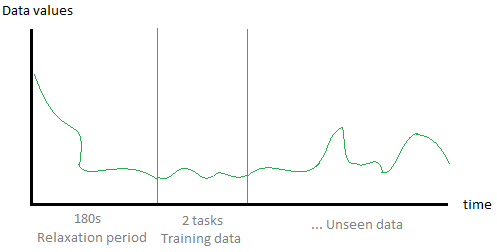
\includegraphics[width=0.95\columnwidth]{graphics/rest_period_training_data.png}
    \caption{The division of the test data parts. The first section is the relaxation period of 180 seconds. The second section is two normal tasks of which the test participants ``normal state'' / baseline is modelled. The last section is the rest of the test, and the section in which frustration is expected in the form of anomalies. }
    \label{[FIGURE] Data Sections}
\end{figure}
\subsection{Feature selection}
% mention related work for [gsr, face, eeg, hr] that looks at frustration or irritation

% UP -> frustatrion -> a / v -> features brugt i papers -> øst og vest -> kigger på features tidligere -> reaction
% kommer instant -> vi bruger derfor de gamle features
Investigating related work for relevant features for capturing frustation, many disparate methods are proposed. However,
we choose to be inspired by the following discoveries.

Poel et al.~\cite{affective_pacman} created ``Affective Pacman'' which induced frustration into the player while allowing synchronous recording of EEG data. After applying a short-term fourier transform and analysing band-power, they found a significant difference in power, between the normal condition and frustrated conditions in the delta and theta bands.

Trogo et al.~\cite{brainwave_signals_frustration} studied the affective state of students. More specifically they looked at boredom, confusion, engagement and frustration. 
A simple application with Berg's Card Sorting Task\cite{bergs_card_sorting} was used as stimuli.
They used the following features on a raw EEG signal: mean, standard deviation, mean of absolute first and second differences and standardized mean of absolute first and second differences.

Harper et al.~\cite{web20_frustration} investigated the frustration induced from the dynamic content of Web 2.0 websites. 
They used GSR to measure frustration levels and found them from peaks in smoothed GSR graphs.

Dang et al.~\cite{stress_robot} used a game to induce stress and had a robot react to the stress levels and try to support the test participant. 
They used heart rate information in form of heart beats per minute to deduce the stress level.

In Edge et al.~\cite{bipolar_frustration} bipolar test participants were studied where anger is a fundamental emotion in the disorder. 
They investigated frustration and irritation as a subset of anger with heart rate variability.

Kosunen et al.~\cite{boredom_negative_mood_features} also used a heart rate sensor.
They found statistic significant features for frustration with intervals of 500-1200ms, to be interbeat-interval(IBI) mean and IBI low frequency/high frequency band power, but also had IBI standard deviation.

Dimberg et al. \cite{face_onset} found unconscious facial reactions happens in the interval 500-1000 ms.
Scherer used ``Facial Action Coding System'' to define and measure facial expressions during an enacted emotion, of which anger and irritation was investigated on an arousal/valence scale~\cite{scherer_kinect}.


\subsubsection{Limitations of current research}
While frustration can be measured, no golden-standard method has been proposed for doing so.  As an example, Zhai et
al.~\cite{gsr_len_lat3} suggests that reactions in GSR can be seen 2-4 seconds after stimuli, and remain observable 3-5
seconds thereafter. This is to say, that in order to capture reactions in GSR, we have to consider \textit{at least}
data within those boundaries. However, Ghaderi et al.~\cite{machine_learning_100s_gsr} proposes durations as long as
100-300 seconds. Likewise, Niemic~\cite{studies_of_emotion} suggests durations of up to 15 seconds for EEG. While such
durations could indeed capture the occurrence of some stimuli, it would prove difficult in our situation as such
durations would likely cover more than just one event. This suggests emotional responses such as frustration, in terms
of researches, can have very different lifetimes depending on the target of research and use case.

Our previous work\cite{first_paper} showed promising results using descriptive statistics, e.g. mean, median and standard deviation. 
As with our previous work, we attempt to capture affective state changes at stimuli exposure. 
As with our first study, the usability problems we deliberately seeded into the test program are of significant severity, and we do not consider problems of cosmetic nature.
Further as the seeded problems can appear within rather short time spans of each other, shorter assumptions of emotions fits the granularity of this study's use case. 
We are inclined to believe the assumption, that a stimuli will have an immediate emotional reaction and a corresponding physiological reaction.
As such, we choose to use the same features as our previous work, with the shortest time durations that literature supports in terms of reaction to measurable physiological changes. 

\subsubsection{Features, latency and duration}
Based on our previous work~\cite{9th_semester_project, first_paper}, with the intent of capturing short-term fleeting
affective changes, we define the following latencies and time-spans to consider for each individual sensor.  We consider
affective state changes in GSR to manifest themselves 2 seconds after the experience occurred which induced the stimuli,
and is noticeable within a time-frame of 5 seconds thereafter, see Table \ref{[TABLE] features gsr}. EEG is considerably
different, manifesting after 350 milliseconds, lasting 710 milliseconds, see Table \ref{[TABLE] features eeg}. Reactions
to stimuli can be seen manifesting in heart-rates after 4 seconds, and lasts for 3 seconds, see Table\ref{[TABLE]
  features hr}.  Lastly face changes has a delay of 500 milliseconds and lasts for 500 milliseconds, see Table
\ref{[TABLE] features face}.

Similar time-frames are also suggested by \cite{eeg_electrodes_0}, which states that reactions lasts for 5
seconds. However, it also suggested that data within 10-15 seconds should be considered - a factor of 2.5.  As stated,
the duration of a response is up for discussion, but in order to consider the fact that emotions potentially spread of a
longer duration of time, we also consider windows which are 2.5 times larger, for each sensor.  This means that for GSR
the window considered would be 10 seconds instead of 5, and similar applies for all sensors.

\begin{table}[H]
    \centering

    {\large \textbf{EEG Features}}\vspace{2pt}
    \begin{tabularx}{\columnwidth}{cXc}
        \toprule
        \textbf{Source} & \textbf{Data captured} & \textbf{Timespan (ms)} \\
        \midrule
        \small{\cite{eeg_music_listening,eeg_timespan_1,eeg_electrodes_1,eeg_electrodes_0}} & AF3-AF4 ($\delta$) & 350 - 1060 \\
        \small{\cite{eeg_music_listening,eeg_timespan_1,eeg_electrodes_1,eeg_electrodes_0}} & AF3-AF4 ($\theta$) & 350 - 1060 \\
        \small{\cite{eeg_music_listening,eeg_timespan_1,eeg_electrodes_1,eeg_electrodes_0}} & AF3-AF4 ($\alpha$) & 350 - 1060 \\
        \small{\cite{eeg_music_listening,eeg_timespan_1,eeg_electrodes_1,eeg_electrodes_0}} & AF3-AF4 ($\beta$)  & 350 - 1060 \\
        \small{\cite{eeg_music_listening,eeg_timespan_1,eeg_electrodes_1,eeg_electrodes_0}} & AF3-AF4 ($\gamma$) & 350 - 1060 \\
        \small{\cite{eeg_music_listening,eeg_timespan_1,eeg_electrodes_1,eeg_electrodes_0}} & F3-F4 ($\delta$) & 350 - 1060 \\
        \small{\cite{eeg_music_listening,eeg_timespan_1,eeg_electrodes_1,eeg_electrodes_0}} & F3-F4 ($\theta$) & 350 - 1060 \\
        \small{\cite{eeg_music_listening,eeg_timespan_1,eeg_electrodes_1,eeg_electrodes_0}} & F3-F4 ($\alpha$) & 350 - 1060 \\
        \small{\cite{eeg_music_listening,eeg_timespan_1,eeg_electrodes_1,eeg_electrodes_0}} & F3-F4 ($\beta$)  & 350 - 1060 \\
        \small{\cite{eeg_music_listening,eeg_timespan_1,eeg_electrodes_1,eeg_electrodes_0}} & F3-F4 ($\gamma$) & 350 - 1060 \\
        \bottomrule
    \end{tabularx}
    % \caption{Timespan is in milliseconds, after stimuli. A indicates the feature can be used to classify arousal and V
    % indicates the same for valence. Only features using electrodes accessible with the Emotiv EPOC were used.}
    \label{[TABLE] features eeg}

    {\large \textbf{GSR Features}}\vspace{2pt}
    \begin{tabularx}{\columnwidth}{cXc}
        \toprule
        \textbf{Source} & \textbf{Data captured} & \textbf{Timespan (ms)}\\
        \midrule
        \cite{gsr_len_lat3, gsr_data_processing} & SD of filtered signal & 2000 - 7000\\
        \cite{gsr_len_lat3, gsr_data_processing} & Mean of filtered signal & 2000 - 7000\\
        \cite{gsr_len_lat3, gsr_data_processing} & Max of filtered signal & 2000 - 7000\\
        \cite{gsr_len_lat3, gsr_data_processing} & Min of filtered signal & 2000 - 7000\\
        \bottomrule
    \end{tabularx}
    %\caption{Timespan is in milliseconds, after stimuli. A indicates the feature can be used to classify arousal and V indicates the same for valence.}
    \label{[TABLE] features gsr}

    {\large \textbf{HR Features}}\vspace{2pt}
    \begin{tabularx}{\columnwidth}{cXc}
        \toprule
        \textbf{Source}                  & \textbf{Data captured} & \textbf{Timespan (ms)} \\
        \midrule
        \cite{hr_feature1, hrv_source_3} & IBI mean               & 4000 - 7000            \\
        \cite{hr_feature1}               & IBI std                & 4000 - 7000            \\
        \cite{hr_feature1}               & HRV RMSSD              & 4000 - 7000            \\
        \bottomrule
    \end{tabularx}
    %\caption{Timespan is in milliseconds, after stimuli. A indicates the feature can be used to classify arousal and V indicates the same for valence.}
    \label{[TABLE] features hr}

    {\large \textbf{Facial Features}}\vspace{2pt}
    \begin{tabularx}{\columnwidth}{cXc}
        \toprule
        \textbf{Source} & \textbf{Data captured} & \textbf{Timespan (ms)} \\
        \midrule
        \cite{scherer_kinect} & Mean of ``eyes closed'' & 500 - 1000 \\
        \cite{scherer_kinect} & SD of ``eyes closed''   & 500 - 1000 \\
        \bottomrule
    \end{tabularx}
    \caption{Timespans are in milliseconds, after some time $t$.}
    \label{[TABLE] features face}
\end{table}